\normalfalse \difficiletrue \tdifficilefalse
\correctiontrue

%\UPSTIidClasse{11} % 11 sup, 12 spé
%\newcommand{\UPSTIidClasse}{11}

\exer{Robot avion  $\star\star$ \label{C2:07:56}}
\setcounter{numques}{0}
\UPSTIcompetence[2]{C2-07}
\index{Compétence C2-07}
\index{PFS}
\index{Robot avion}
\ifcorrection
\else
\textbf{Pas de corrigé pour cet exercice.}
\fi

\ifprof
\else

\begin{obj}
L'objectif est de déterminer le couple articulaire $C_{12}$ à appliquer sur le bras 2 afin de garantir l'effort de
perçage et l’effort presseur.
\end{obj}


\begin{center}
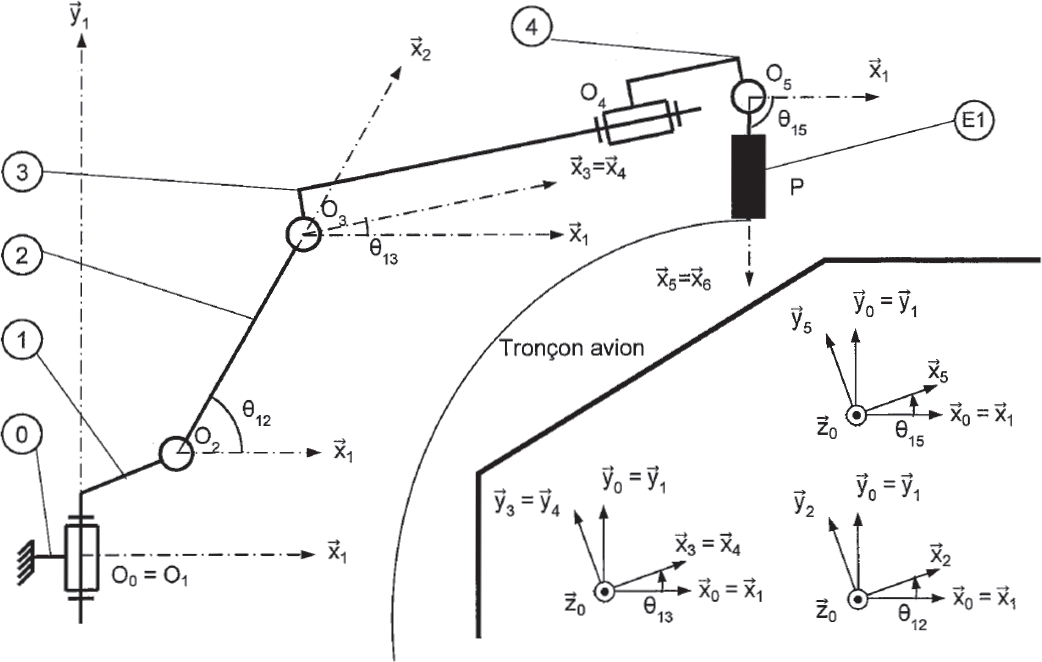
\includegraphics[width=\linewidth]{56_01}
\end{center}


\textbf{Hypothèses :}
\begin{itemize}
\item l'étude est réalisée pour une demi couture orbitale (couture supérieure);
\item le repère $\rep{0}\repere{O_0}{x_0}{y_0}{z_0}$ sera supposé galiléen;
\item $\vect{y_0}$ est l’axe vertical ascendant et $\vect{g}=-g\vect{y_0}$ avec $g = \SI{9,81}{m.s^{-2}}$;
\item toutes les liaisons sont supposées parfaites.
\end{itemize}



\textbf{Repérage et paramétrage}

Le repère associé à l'embase fixe (0) est le repère $\rep{0}\repere{O_0}{x_0}{y_0}{z_0}$, $\vect{y_0}$ étant l'axe vertical
ascendant.

L'embase de rotation (1), en liaison pivot d'axe $\axe{O_1}{y_1}$, par rapport au bâti (0), a pour repère
associé le repère $\rep{1}\repere{O_1}{x_1}{y_1}{z_1}$ tel que $O_0=O_1$, $\vect{x_0}=\vect{x_1}$, $\vect{y_0}=\vect{y_1}$, $\vect{z_0}=\vect{z_1}$.

Le bras (2), en liaison pivot d'axe $\axe{O_2}{z_2}$ par rapport à l’embase de rotation (1), a pour repère
associé le repère $\rep{2}\repere{O_2}{x_2}{y_2}{z_2}$ tel que $\vect{O_1 O_2} = L_1\vect{x_1} + L_2\vect{y_1}$, $\vect{z_1}=\vect{z_2}$ et $\angl{x_1}{x_2}=\angl{y_1}{y_2}=\theta_{12}$.

Le bras (3), en liaison pivot d'axe $\axe{O_3}{z_3}$ par rapport au bras (2), a pour repère
associé le repère $\rep{3}\repere{O_3}{x_3}{y_3}{z_3}$ tel que $\vect{O_2 O_3} = L_3\vect{x_2} $, $\vect{z_1}=\vect{z_3}$ et $\angl{x_1}{x_3}=\angl{y_1}{y_3}=\theta_{13}$.


Le bras (4), en liaison pivot d'axe $\axe{O_4}{x_4}$ par rapport au bras (3), a pour repère
associé le repère $\rep{4}\repere{O_4}{x_4}{y_4}{z_4}$ tel que $\vect{O_3 O_4} = L_4\vect{x_3} +l_5 \vect{y_3}$, $\vect{x_3}=\vect{x_4}$ et $\angl{y_3}{y_4}=\angl{z_3}{z_4}=\theta_{34}$.

L'ensemble (E1) composé du bras (5), du poignet et de l'outil, en liaison pivot d'axe $\axe{O_5}{z_5}$ par
rapport au bras (4), a pour repère associé le repère $\rep{5}\repere{O_5}{x_5}{y_5}{z_5}$ tel que $\vect{O_4O_5}=L_5\vect{x_3}$, $\vect{z_1}=\vect{z_5}$ et $\angl{x_1}{x_5}=\angl{y_1}{y_5}=\theta_{15}$.


La masse du bras (2) est notée $M_2$ et la position du centre de gravité est définie par $\vect{O_2G_2}=\dfrac{1}{2}L_3\vect{x_2}$.


La masse du bras (3) et du bras (4) est notée $M_{34}$ et la position du centre de gravité est définie par
$\vect{O_3G_3}=\dfrac{1}{3}L_4\vect{x_3}+L_5\vect{y_3}$.

La masse de l'ensemble (E1) est notée $M_{E1}$ et la position du centre de gravité est définie par
$\vect{O_5G_5}=L_7\vect{x_5}$. 

L’extrémité de l’outil est définie par le point $P$ définie par $\vect{O_5P}=L_8\vect{x_5}$. 

Le torseur d’action mécanique lié au perçage sera noté : $\torseurstat{T}{\text{Tronçon (perçage)}}{E_1}=\torseurcol{-F}{0}{0}{0}{0}{0}{P, \rep{5}}$.
Un effort presseur est de plus nécessaire pour le perçage optimal des deux tronçons. Le torseur
d’action mécanique associé sera noté : $\torseurstat{T}{\text{Tronçon (presseur)}}{E_1}=\torseurcol{-P}{0}{0}{0}{0}{0}{P, \rep{5}}$.

Le torseur couple modélisant l'action du moteur sur la pièce \textbf{1} sur \textbf{2} : $\torseurstat{T}{1_m}{2}=\torseurl{\vect{0}}{C_{12}\vect{z_0}}{\forall P}$.


La rotation entre les solides (0) et (1) est supposée bloquée dans la suite du sujet.


\fi

\question{Réaliser le graphe de structure de l'ensemble en précisant les liaisons et les actions mécaniques extérieures.}
\ifprof
\begin{center}
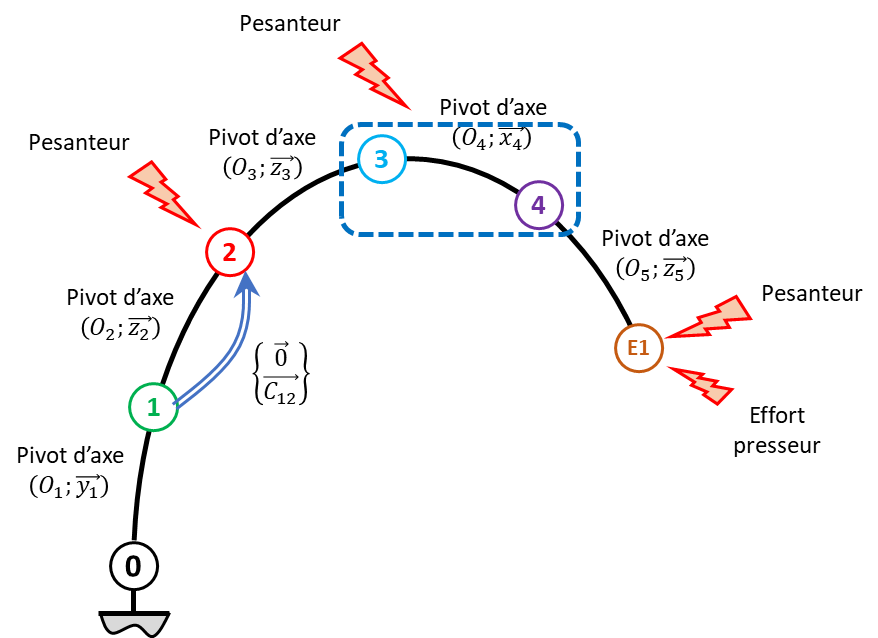
\includegraphics[width=.5\linewidth]{56_01_cor}
\end{center}
\else
\fi

\question{Quel est l'ensemble $\Sigma$ à isoler afin de déterminer le couple $C_{12}$.}

\ifprof
En isolant l'ensemble $\Sigma = \{2+3+4+E_1\}$ on ne fera apparaître \textbf{QUE} $C_{12}$ et les actions mécaniques extérieures. Les actions de liaison 2--3, 3--4, 4--E1 \textbf{n'interviendont pas}. 
\else
\fi

\question{Réaliser un bilan des actions mécaniques extérieures appliquées à $\Sigma$ et écrire les éléments de réduction de chaque torseur d'actions mécaniques.}
\ifprof
\begin{center}
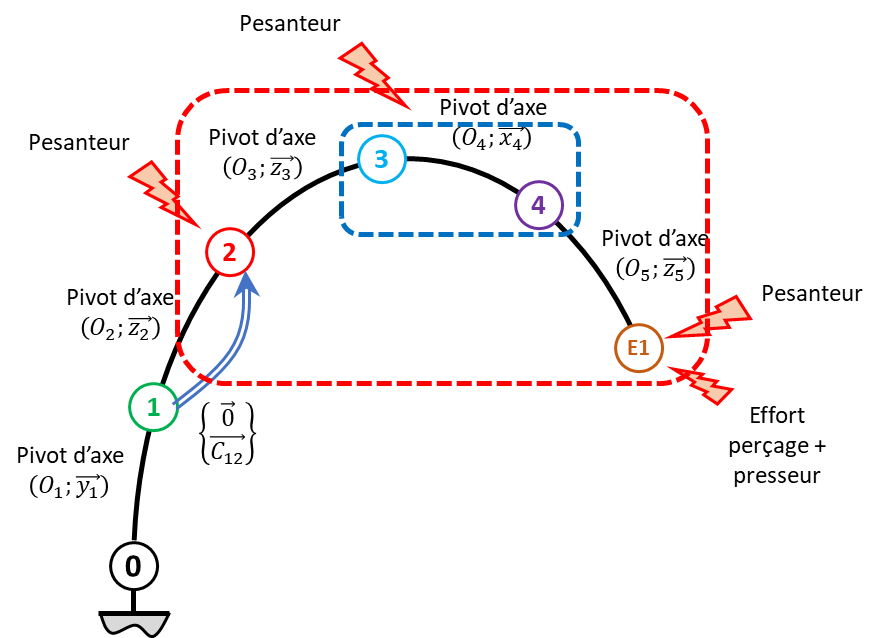
\includegraphics[width=.5\linewidth]{56_02_cor}
\end{center}
Bilan des actions mécaniques :
\begin{itemize}
\item pivot 1--2  et couple moteur de 1 sur 2;

\item pesanteur sur 2 : $\torseurstat{T}{\text{pes}}{2}$ $=\torseurl{-M_2g \vect{y_1} }{\vect{0}}{G_2}$.
On a par ailleurs $\vectm{O_2}{\text{pes}}{2} = \vect{O_2 G_2} \wedge-M_2g \vect{y_1}$
$= \dfrac{1}{2}L_3\vect{x_2} \wedge-M_2g \vect{y_1}$
$= -\dfrac{1}{2}M_2gL_3 \cos \theta_{12} \vect{z_0} $;

\item pesanteur sur 3 et 4 : $\torseurstat{T}{\text{pes}}{3+4}$ $=\torseurl{-M_{34} g \vect{y_1} }{\vect{0}}{G_3}$.
On a par ailleurs $\vectm{O_2}{\text{pes}}{3+4} = \vect{O_2 G_3} \wedge-M_{34}g \vect{y_1}$
$= \left( L_3\vect{x_2} +\dfrac{1}{3}L_4\vect{x_3}+L_5\vect{y_3}\right) \wedge-M_{34}g \vect{y_1}$
$= -M_{34}g\left( L_3\vect{x_2}\wedge \vect{y_1} +\dfrac{1}{3}L_4\vect{x_3}\wedge \vect{y_1}+L_5\vect{y_3}\wedge \vect{y_1} \right) $
$= -M_{34}g\left( L_3\cos\theta_{12} +\dfrac{1}{3}L_4\cos\theta_{12}-L_5\sin\theta_{13}\right) \vect{z_0}$;

\item pesanteur sur $E_1$ : $\torseurstat{T}{\text{pes}}{E1}$ $=\torseurl{-M_{E1} g \vect{y_1} }{\vect{0}}{G_5}$.
On a par ailleurs $\vectm{O_2}{\text{pes}}{E1} = \vect{O_2 G_5} \wedge-M_{E1}g \vect{y_1}$;
$= -M_{E1}g\left( L_3 \vect{x_2}+L_4\vect{x_3}+L_5 \vect{x_3}+l_5 \vect{y_3}+L_7 \vect{x_5} \right)\wedge \vect{y_1}$
$= -M_{E1}g\left( L_3 \cos\theta_{12}+L_4\cos\theta_{13}+L_5 \cos\theta_{13}-l_5 \sin\theta_{13}+L_7 \cos\theta_{15}\right) \vect{z_0}$;


\item effort presseur + perçage $\torseurstat{T}{\text{Tronçon }}{E_1}=\torseurcol{-F-P}{0}{0}{0}{0}{0}{P, \rep{5}}$.
On a par ailleurs $\vectm{O_2}{\text{Tronçon}}{E1} = \vect{O_2 P} \wedge(-F-P) \vect{x_5}$
$= \left(  L_3 \vect{x_2}+L_4\vect{x_3}+L_5 \vect{x_3}+l_5 \vect{y_3}+L_8 \vect{x_5} \right)\wedge(-F-P) \vect{x_5}$
$= -(F+P)\left(  L_3 \vect{x_2}\wedge \vect{x_5}+L_4\vect{x_3}\wedge \vect{x_5}+L_5 \vect{x_3}\wedge \vect{x_5}+l_5 \vect{y_3}\wedge \vect{x_5} \right)\wedge $
$= -(F+P)\left(  L_3 \sin\left(\theta_{15}-\theta_{12} \right)+ \left(L_4+L_5\right)\sin\left(\theta_{15}-\theta_{13} \right)+l_5 \sin\left(\theta_{15}-\theta_{13} -\dfrac{\pi}{2} \right)  \right)\vect{z_0}$.
\end{itemize}
\else
\fi

\question{Quel théorème doit-être appliqué et sur quel axe de projection, pour déterminer le couple $C_{12}$ ?}
\ifprof
Pour ne pas faire apparaître les actions de la liaison 1--2 il faudra réaliser un théorème du moment statique en $O_2$ en projection sur $\vect{z_2}$ (la liaison pivot n'a pas de composante en ce point et sur cette projection).

On a donc : 
$
 -\dfrac{1}{2}M_2gL_3 \cos \theta_{12}
  -M_{34}g\left( L_3\cos\theta_{12} +\dfrac{1}{3}L_4\cos\theta_{12}-L_5\sin\theta_{13}\right)
  -M_{E1}g\left( L_3 \cos\theta_{12}+L_4\cos\theta_{13}+L_5 \cos\theta_{13}-l_5 \sin\theta_{13}+L_7 \cos\theta_{15}\right) 
  -(F+P)\left(  L_3 \sin\left(\theta_{15}-\theta_{12} \right)+ \left(L_4+L_5\right)\sin\left(\theta_{15}-\theta_{13} \right)+l_5 \sin\left(\theta_{15}-\theta_{13} -\dfrac{\pi}{2} \right)  \right) 
  = 0
$.
\else
\fi


\ifprof
\else
La configuration correspondant à la position extrême supérieure de la couture orbitale correspond aux angles suivants : $\theta_{12}=\SI{60}{\degres}$, $\theta_{13}=-\SI{4}{\degres}$, $\theta_{15}=-\SI{90}{\degres}$.

Dans la suite de l'étude, l'angle $\theta_{13}$ sera considéré nul.
\fi

\question{Déterminer l'équation littérale du couple $C_{12}$ en fonction de $g$, $F$, $P$, $M_2$, $M_{34}$, $M_{E1}$, $L_3$, $L_4$, $L_5$, $L_6$, $L_7$, $\theta_{12}$, $\theta_{15}$.}
\ifprof
On a 
$
C_{12} -\dfrac{1}{2}M_2gL_3 \cos \theta_{12}
  -M_{34}g\left( L_3\cos\theta_{12} +\dfrac{1}{3}L_4\cos\theta_{12}\right)
  -M_{E1}g\left( L_3 \cos\theta_{12}+L_4+L_5+L_7 \cos\theta_{15}\right) 
  -(F+P)\left(  L_3 \sin\left(\theta_{15}-\theta_{12} \right)+ \left(L_4+L_5\right)\sin\left(\theta_{15} \right)-l_5 \cos\left(\theta_{15}  \right)  \right) 
  = 0
$.
\else
\fi

Les valeurs du robot considéré sont :
\begin{itemize}
\item $M_{2}=\SI{264}{kg}$, $M_{34}=\SI{430}{kg}$, $M_{\text{E1}}=\SI{150}{kg}$, $P=\SI{150}{N}$, $F=\SI{1000}{N}$;
\item $L_{1}=\SI{0,405}{m}$, $L_{2}=\SI{0,433}{m}$, $L_{3}=\SI{1,075}{m}$, $L_{4}=\SI{1,762}{m}$, $L_{5}=\SI{0,165}{m}$, $L_{6}=\SI{0,250}{m}$, $L_{7}=\SI{0,550}{m}$, $L_{8}=\SI{0,750}{m}$.
\end{itemize}

\question{Déterminer alors la valeur du couple~$C_{12}$.}
\ifprof
On a 
$
C_{12} -\dfrac{1}{2}M_2gL_3 \cos \theta_{12}
  -M_{34}g\left( L_3\cos\theta_{12} +\dfrac{1}{3}L_4\cos\theta_{12}\right)
  -M_{E1}g\left( L_3 \cos\theta_{12}+L_4+L_5 \right) 
  -(F+P)\left(  L_3 \cos\left(\theta_{12} \right)- \left(L_4+L_5\right)  \right) 
  = 0
$.
Soit 
$
C_{12} -\dfrac{1}{4}M_2gL_3 
  -M_{34}g\dfrac{1}{2}\left( L_3 +\dfrac{1}{3}L_4\right)
  -M_{E1}g\left( L_3 \dfrac{1}{2}+L_4+L_5 \right) 
  -(F+P)\left(  L_3 \dfrac{1}{2}- \left(L_4+L_5\right)  \right) 
  = 0
$.
Au final 
$
C_{12} 
= \dfrac{1}{4}M_2gL_3 
  +M_{34}g\dfrac{1}{2}\left( L_3 +\dfrac{1}{3}L_4\right)
  +M_{E1}g\left( L_3 \dfrac{1}{2}+L_4+L_5 \right) 
  +(F+P)\left(  L_3 \dfrac{1}{2}- \left(L_4+L_5\right)  \right) 
$.
\else
\fi


La valeur limite supérieure du couple $C_{12}$ est fixée par le constructeur à \SI{9000}{Nm}.

\question{Le choix du robot permettra-t-il de garantir les conditions d'assemblage dans cette position ? Justifier la réponse. }
\ifprof
 $C_{12} = \SI{6230}{Nm}$. Compatible avec le cahier des charges. 
\else
\fi







\ifprof
\else
\begin{flushright}
\footnotesize{Corrigé  voir \ref{C2:07:56}.}
\end{flushright}%
\fi 